\section{Introduction}\label{section:intro}
Measurements play a fundamental role in generating observations and
are indispensable to any inference process. Selecting the optimal set
of measurements holds particular significance when inferring
parameters of a physical process. Unlike many other fields, where
measurements are fixed, in this context, we have the freedom to choose
which measurements to take. This freedom should be taken advantage of:
measurements should be chosen to enhance accuracy, reduce costs, or
both. Whether measurements involve specifying electrode locations on
the skin in electric impedance tomography \cite{horesh2010impedance},
determining certain wavelengths in MRI \cite{horesh2008mri},
positioning sensors for detecting ground-reflected waves in the search
for oil \cite{horesh2008borehole}, or optimizing sensor locations in a
seismographic network \cite{rabinowitz1990, steinberg1995} --- the
selection of optimal measurements, referred to as the problem of
\emph{optimal design}, becomes crucial. Optimal measurements are
chosen according to specific \emph{design criteria}, with A- and
D-optimality being two of the most widely recognized and extensively
studied design criteria \cite{Chaloner1995,
  AlexanderianGloorGhattas14}.


Surprisingly, A- and D-optimal designs have been observed to yield
remarkably similar measurements in certain cases \cite{fedorov1996,
  nyberg2012, fedorov1997, Ucinski05, neitzel2019sparse}. To
illustrate this point, we consider a toy problem: inferring
the initial condition of the 1D heat equation (details in the
supplementary material). In Fig.~\ref{fig:clusterization
  illustration} D-optimal measurement locations are shown for
different numbers of measurements. Notably, for six measurements, a
D-optimal design yields two sets of measurements that are almost
indistinguishable from one another. We refer to this intriguing
phenomenon as \emph{measurement clusterization} \cite{Ucinski05}, and
we refer to a design that exhibits measurement clusterization as a
\emph{clustered design}.


%% first: blue, second: red, third: green, fourth: black,
%% fifth:magenta
\begin{figure}
    \centering
    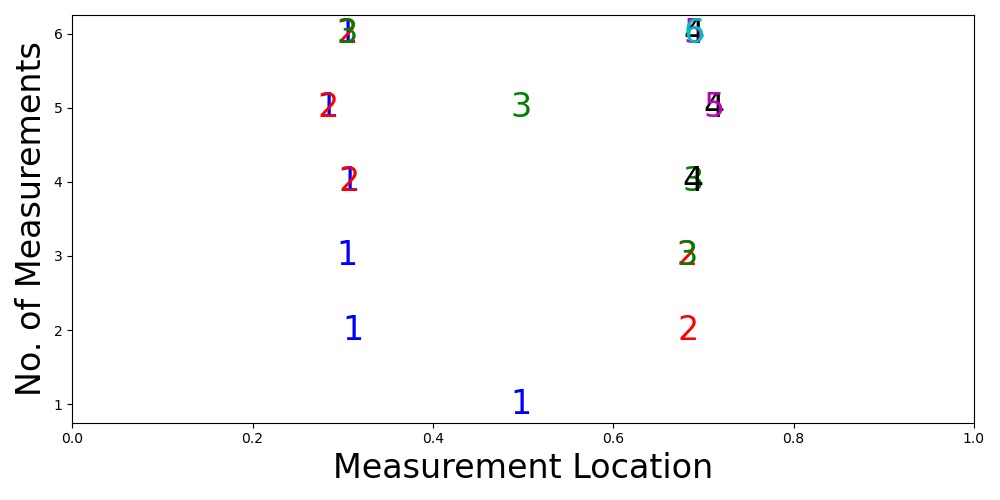
\includegraphics[height=0.5\textwidth]{example.png}
    \caption{Measurement clusterization for optimal designs when
      inverting for the initial condition of the 1D heat equation (see
      supplementary material for details). Measurement locations were
      chosen according to the Bayesian D-optimality criterion of
      Theorem \ref{thm:d optimality}. Measurement locations are
      plotted over the computational domain \(\Omega = [0, 1]\)
      (x-axis), for varying numbers of measurements (y-axis). The
      colored numbers are measurement indices, plotted for visual
      clarity. Measurement clusterization already occurs for three
      measurements: the second measurement (red) is overlaid with the
      third (green). For five measurements, first (blue) and second
      (red) measurements are clustered, as well as the fourth (black)
      and the fifth (magenta).}
  \label{fig:clusterization illustration}
\end{figure}


Researchers widely agree that measurement clusterization is
undesirable \cite{fedorov1996, nyberg2012, fedorov1997, Ucinski05,
  neitzel2019sparse}, prompting the exploration of various remedies to
address this issue. One approach involves merging close measurements
\cite{fedorov1997}; however, this strategy merely overlooks the
phenomenon of measurement clusterization. An alternative solution lies
in \emph{clusterization-free design}s, where measurement locations are
deliberately chosen to be distant from one another. This can be
achieved by imposing distance constraints between measurements or by
introducing correlated errors that account for both observation error
and model misspecification \cite{Ucinski05}. For instance, in the
context of time-series analysis for pharmacokinetic experiments,
measurement clusterization can be mitigated by incorporating the
modeling of auto-correlation time within the noise terms
\cite{nyberg2012}.


In spatial problems involving choice of measurements within a domain
\(\Omega \subseteq \mathbb{R}^d, d=1,2,3\), many researchers
circumvent the problem of measurement clusterization by choosing
measurements from a coarse grid in \(\Omega\) \cite{koval2020,
  alexanderian2021, attia2022, alexanderian2014, alexanderian2016,
  alexanderian2018efficient, brunton2016}. This approach incurs a
significant computational cost as it requires solving a difficult
combinatorial optimization problem for measurement locations over a
finite set. The combinatorial optimization problem is usually relaxed
by first assigning optimal measurement weights in \(\mathbb{R}_+\) to
the potential measurement locations. Some researchers incorporate a
sparsifying \(\ell_1\) penalty term into the design criterion, which
is subsequently thresholded to achieve the desired binary design over
the coarse grid \cite{horesh2008borehole}. Others progressively relax
the \(\ell_1\) penalty to an \(\ell_0\) penalty via a continuation
method \cite{alexanderian2016, alexanderian2014}. Others cast the
problem of finding optimal measurement weights as a stochastic
optimization problem \cite{attia2022stochastic}. All of the
aforementioned methods may indeed find a binary optimal design
restricted to a given coarse grid. However, none addresses one
fundamental issue: the restriction of measurement locations to a
coarse grid in \(\Omega\) fundamentally changes the optimal design
problem and thus results in a sub-optimal design.

Avoiding measurement clusterization is a pragmatic approach:
intuitively, researchers recognize that measurement clusterization is
undesirable, even though the underlying reasons may not be fully
clear. Consequently, they strive to prevent it and devise various
methodologies to avoid measurement clusterization. Yet each and every
one of these methodologies achieves its objective by imposing
restrictions on measurement locations, thereby fundamentally altering
the optimal design problem. To the best of my knowledge, no previous
study has tried to address some seemingly simple yet fundamental
questions:
%
Why does imposing correlations between observations alleviate
measurement clusterization?
%
Is measurement clusterization a generic phenomenon?
%
And, most importantly: Why does measurement clusterization occur?
%
%Should we aim to avoid measurement clusterization?
%
%Is it possible to substitute an optimal clustered design with an
%equally optimal non-clustered design?
%Can an optimal clustered design be relpaced with an equally optimal
%non-clustered design?


\subsection{Contribution}
The primary objective of this study is to provide a comprehensive
understanding of measurement clusterization by addressing the
aforementioned questions. Our focus centers around investigating the
Bayesian D-optimality criterion, which involves maximizing the
expected Kullback-Leibler divergence between the posterior and prior
measures \cite{CoverThomas91, Chaloner1995}. We conduct an analysis of
Bayesian D-optimal designs within the context of linear inverse
problems over Hilbert spaces. We propose a novel relaxed model for
D-optimality that maintains analytical tractability and enables the
identification of D-optimal designs using Lagrange multipliers. This
analytical framework facilitates the exploration of the questions
posed at the end of the previous paragraph:

\begin{figure}
    \centering
    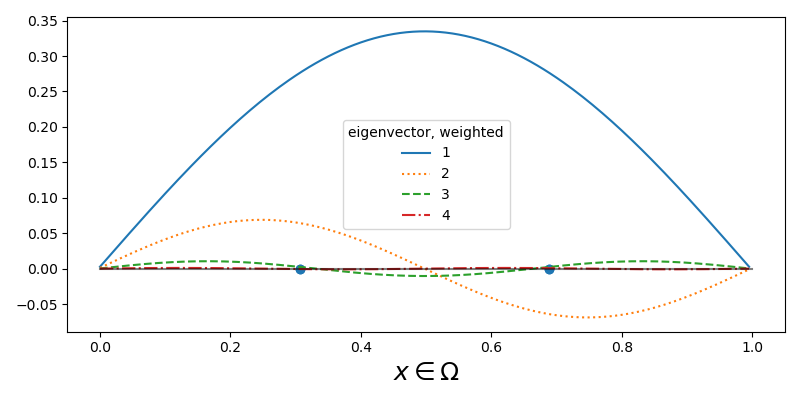
\includegraphics[width=\textwidth]{eigenvectors.png}
    \caption{D-optimal measurement locations ($m=4$ measurements) and
      weighted eigenvectors for finding the initial condition of
      the 1D heat equation. Measurement locations and weighted
      eigenvectors are plotted over the computational domain $\Omega =
      [0, 1]$ (x-axis). Measurement clusterization occurs
      approximately at $0.31$ and $0.69$. These two locations are a
      compromise between zeros of eigenvectors a D-optimal design aims
      to ignore (third and up) and staying far from zeros of the
      eigenvectors a D-optimal design aims to measure (first and
      second). Allocating $m=4$ measurements into two locations
      results in clusterization, according to the pigeonhole
      principle.}
  \label{fig:why}
\end{figure}

\begin{enumerate}

\item \label{q:generic} \textbf{Is measurement clusterization a
  generic phenomenon?}
  %\subsection{An answer for Question \ref{q:generic}: Genericity of measurement clusterization}
  %% Computer implementation of Lemma \ref{thm:char} for the inverse
  %% problem outlined in Section \ref{section:how} also generates \(\obs\)
  %% as a solution to the D-optimal design problem.  Furthermore,
  Randomized numerical simulations of our model give rise to D-optimal
  designs that exhibit clusterization more than 95\% of the time (see
  code in supplementary material). Given our model's genericity, we
  expect measurement clusterization to be a generic phenomenon.

\item \label{q:mitigate} \textbf{Why does imposing correlations
  between observations alleviate measurement clusterization?} In
  Section \ref{section:non vanishing}, we rigorously demonstrate the
  role of model error in mitigating clusterization, thereby
  corroborating earlier observations made by various researchers.

\item \label{q:why} \textbf{Why does measurement clusterization
  occur?} In Section \ref{section:why}, we present a compelling
  explanation for the optimality of clustered designs in the absence
  of model error. Our analysis reveals that, in our model, a D-optimal
  design focuses on a select set of prior eigenvectors, specifically
  those with the largest eigenvalues in the prior covariance
  spectrum. In practical scenarios, the number of locations where (a)
  the relevant prior eigenvectors are significantly large, and (b)
  other eigenvectors are close to zero, is limited. Consequently, the
  clusterization of measurements arises as a natural consequence of
  the pigeonhole principle, as there are more measurements available
  than there are locations satisfying conditions (a) and (b). See
  Fig~\ref{fig:why}.


  %% In Section \ref{section:vanishing}, we provide an insightful
  %% explanation for the optimality of clustered designs when no model
  %% error is present. We demonstrate that for our model, a D-optimal
  %% design measures only a small subset of prior eigenvectors, which are
  %% the prior eigenvectors with largest power spectrum. In real-life
  %% problems there are limited number of locations where: (a) the
  %% relevant prior eigenvectors are large, and other prior eigenvectors
  %% with large power in the prior spectrum are zero. Then measurement
  %% clusterization is a result of the pigeonhole principle, where there
  %% are more measurements than measurement locations satisfying (a) and
  %% (b).

  %% We conjecture that the prevalence of measurement clusterization
  %% arises due to the ease of discovering clustered designs.


%% \item \label{q:avoid} \textbf{Should we aim to avoid measurement
%%   clusterization?} Based on the analysis conducted in this study, we
%%   did not find any compelling reason to explicitly avoid optimal
%%   clustered designs.

%% \item \label{q:replace} \textbf{Is it possible to substitute an
%%   optimal clustered design with an equally optimal non-clustered
%%   design?} In Section \ref{section:vanishing}, we answer this question
%%   in the affirmative, although we show that numerical experiments
%%   conducted using our model indicate a strong preference for clustered
%%   designs.

\end{enumerate}

The cornerstone of our investigation into measurement clusterization
is Theorem \ref{thm:char} proven in Section
\ref{section:vanishing}. The key insight of Theorem \ref{thm:char}
lies in its fifth component, which highlights that a D-optimal design
aims to uniformly reduce posterior uncertainties for posterior
covariance eigenvectors in observation space. A similar conclusion was
reached by Koval et al.~\cite{koval2020}, who showed that A-optimal
designs are best constructed in the space of observations.

Before we state Theorem \ref{thm:char} we give some definitions: Let
\(\hilp, \hilo\) Hilbert spaces, \(\fwd:\hilp \to \hilo\) a linear
compact operator. Let \(\obs: \hilo \to \mathbb{R}^m\) a linear
measurement operator, where \(m \in \mathbb{N}\) is the number of
measurements taken. Let \(\sigma^2 \in \mathbb{R}_{+}\) observation
noise variance, \(\data = \obs \fwd \param + \eps\), where \(\eps \in
\mathbb{R}^m\) is iid \(\mathcal{N}(0, \sigma^2)\) noise. Let \(\pr
\sim \mathcal{N}(\prmean, \prcov)\) prior Gaussian measure on
\(\hilp\), where \(\prcov\) is the prior covariance operator and let
\(\post\) the posterior (Gaussian) measure.
  
\begin{restatable}{theorem}{char}\label{thm:char}
  Let:
  \begin{itemize}
    \item The D-optimality design criterion
    \cite{AlexanderianGloorGhattas14}:
    \begin{align*}
      \begin{split}
        \tar(\obs) %:&= \mathbb{E}_{\data}\left [ D_{\text{KL}} (\post || \pr ) \right ] \\
        % 
        % 
        % 
        &= \frac12 \log \det ( I + \sigma^{-2} \prcov^{1/2} \fwd ^*
        \obs^* \obs \fwd \prcov^{1/2}), 
      \end{split}
    \end{align*}
  \item \(\obs\) a D-optimal design operator
    \begin{equation*}
      \obs = \argmax_{\|\meas_j\| = 1, j=1,\dots,m}\tar(\obs),
    \end{equation*}
  \item \(\{\lambda_i\}_{i=1}^\infty\) eigenvalues of
    \(\fwd\prcov\fwd^*\) in decreasing order of magnitude.
    %% \item \(\{\ev_i\}_{i=1}^\infty\) their corresponding eigenvectors.
  \item \(\{\eta_i\}_{i=1}^\infty\) eigenvalues of \(\obs^*\obs\).
 
  \end{itemize}

  Then:
  \begin{enumerate}
  \item  \(\tr{\obs^*\obs} = m\).
  \item \(\obs^*\obs\) and \(\fwd\prcov\fwd^*\) are simultaneously
    diagonalizable.
  \item \(k := \rank \obs^*\obs \leq m\) and
    \begin{equation*}
      \tar(\obs) = \frac12 \sum_{i=1}^{k} \log (1 + \sigma^{-2}\lambda_i\eta_i). %= \frac12 \sum_{i=1}^{m} \log (1 + \sigma^{-2}\lambda_i\eta_i).
    \end{equation*}
  %% \item 
  %%   \begin{equation*}
  %%     k = \argmax \left \{ k:\lambda_k^{-1} < \sigma^{-2}\frac{m}{k} + \frac{1}{k} \sum_{j=1}^{k}
  %%     \lambda_j^{-1} \right \}.
  %%   \end{equation*}
  \item
    \begin{equation*}
        \eta_i = \begin{cases}
          \frac{m}{k} - \sigma^2 \lambda_i^{-1} + \sigma^2 \frac{1}{k} \sum_{j=1}^k \lambda_j^{-1} & 1 \leq i \leq k \\
          0 & i > k 
        \end{cases}.
    \end{equation*}
  \item The covariance of the pushforwad \(\fwd_{*} \post\) is \(\left
    ( (\fwd \prcov \fwd^*)^{-1} + \sigma^{-2} \obs^*\obs \right
    )^{-1}\) and its eigenvalues are
    \begin{equation*}
      \theta_i =
      \begin{cases}
        \left(\frac{\sum_{j=1}^k \lambda_j^{-1} + \sigma^{-2}m}{k} \right )^{-1} & i \leq k \\
        \lambda_i &  i > k 
      \end{cases}
    \end{equation*}
  \end{enumerate}
%\end{theorem}
\end{restatable}

In the process of proving Theorem \ref{thm:char} we prove and
generalize several lemmas. Among those, is Lemma \ref{lemma:free},
which is (to the the best of my knowledge) a novel lemma in linear
algebra: We decompose a symmetric positive definite matrix \(M \in
\mathbb{R}^{k \times k}\) with \(\ttr M = m \in \mathbb{N}\) as \(M =
AA^t\), where \(A\) has unit norm columns.

%% Finally, in Lemma \ref{lemma:lax} we generalize a lemma for
%% calculating \(\frac{\der}{\der t} \log \det (I + X(t))\), where
%% \(X(t)\)is an operator valued function \cite{Lax07}.

\subsection{Limitations}\label{subsec:limitations}
The main limitation of this study is that our generic model does not
correspond to any specific real-life problem. It is generic enough to
be analytically tractable, but one may argue our model is too far
removed from any real application. To these claims I would answer that
scientists have a long history of studying models that are bare-bones
simplifications of real systems, e.g. the Ising model
\cite{cipra1987}, the Lorenz system \cite{brin}, the Lotka-Volterra
equations \cite{logan2006}, the Carnot engine \cite{kardar2007}, and
many others.
